\documentclass{article}

% Encoding and Geometry
\usepackage[utf8]{inputenc}
\usepackage[a4paper, margin=1in]{geometry} % Standard 1-inch margins for better layout
\usepackage{parskip}

% Math Packages
\usepackage{amsmath, amsfonts, mathtools}

% Graphics and Figures
\usepackage{graphicx}
\usepackage{caption}
\usepackage{subcaption}
\usepackage{multirow}
\usepackage{tikz}
\usetikzlibrary{positioning} % Ensures compatibility with Overleaf

% Hyperlinks
\usepackage[colorlinks=true, linkcolor=blue, urlcolor=blue]{hyperref} % Load last to avoid conflicts

% Floating Objects Placement
\usepackage[section]{placeins} 

% Bibliography
\usepackage[
    backend=biber,
    style=alphabetic,
    sorting=ynt
]{biblatex}
\addbibresource{references.bib}

% Title Information
\title{EulerSwap White Paper}
\author{Euler Labs}
\date{February 2025}

\begin{document}

\maketitle

\begin{abstract}    
EulerSwap is an automated market maker (AMM) that integrates with Euler credit vaults to provide deeper liquidity for swaps. When a user initiates a swap, a smart contract called an EulerSwap operator borrows the required output token using the input token as collateral. This model enables up to 40x the liquidity depth of traditional AMMs by making idle assets in Euler more efficient. Unlike traditional AMMs, which often fragment liquidity across multiple pools, EulerSwap further increases capital efficiency by allowing a single, cross-collateralised credit vault to support multiple asset pairs at once. At its core, EulerSwap uses a flexible AMM curve to optimise swap pricing, ensuring deep liquidity while maintaining market balance. By combining just-in-time liquidity, shared liquidity across pools, and customisable AMM mechanics, EulerSwap reduces inefficiencies in liquidity provision, offering deeper markets, lower costs, and greater control for liquidity providers.
\end{abstract}

\section{Introduction}

EulerSwap is an automated market maker (AMM) that leverages Euler credit vaults for the provision of just-in-time liquidity as a way to provide deeper liquidity for swaps. EulerSwap differs from traditional AMMs in that it does not depend on many small liquidity providers (LPs) pooling their liquidity inside a single contract. Instead, each EulerSwap instance has a single LP -- an account holder on Euler -- whose deposits function as both liquidity for swaps and as margin collateral for building leveraged positions inside Euler. 

When a user initiates a swap, EulerSwap dynamically borrows the required `out token' using the `in token' and the LP's initial margin collateral as backing. This borrowing approach ensures liquidity is provided just-in-time, only when needed, maximising capital efficiency. By borrowing liquidity to service swaps in this way, EulerSwap can turn \$1M initial liquidity into the equivalent of a \$40m deep liquidity pool on a traditional AMM (see Example below).

The way this works under the hood is by taking advantage of the `operator' functionality of the Ethereum Vault Connector (EVC), which provides a way for Euler credit vault users to delegate authority to someone else to manage their account balances. An EulerSwap operator is a smart contract that manages an LP's account on their behalf using the logic encoded in a custom-built AMM smart contract. Specifically, an EulerSwap operator is able to rebalance the collateral and debt inside an LPs account in order to service swaps and earn swap fees.

Unlike conventional AMMs, which usually require separate liquidity pools for each asset pair, EulerSwap further increases capital efficiency by enabling the use of a single, cross-collateralised credit vault to support multiple asset pairs at once. This liquidity-sharing model ensures that idle liquidity can be used efficiently across multiple trading pairs simultaneously. This design resembles Curve's 3pool concept, but extends it to any number of asset pairings. Unlike traditional AMMs that silo liquidity into separate pools, EulerSwap's cross-collateralisation allows a single USDC credit vault to back multiple trading pairs simultaneously, maximising liquidity utilisation. A single USDC credit vault could be used to support swaps with USDT, USDE, DAI, and many other pairs all in the same block.

EulerSwap introduces a flexible AMM curve (illustrated in Figure \ref{fig:fig1}) that supports deep liquidity for short-term swaps while maintaining a neutral net position over longer periods. A highly customisable curve allows for bespoke pricing strategies, asymmetric liquidity deposits, and single-sided liquidity concentration—all fully controlled by the LP. LPs can modify their EulerSwap parameters at any time by simply swapping out the operator smart contract in their Euler account for another one.

For end-users, EulerSwap offers a seamless, Uniswap-style experience, while behind the scenes, it harnesses advanced features such as dynamic liquidity borrowing, custom pricing curves, and shared liquidity provisioning. Liquidity providers, including professional market makers, token issuers, and DAOs, gain unprecedented capital efficiency. Meanwhile, swappers—ranging from leverage traders and aggregators to MEV bots—benefit from deeper liquidity and optimised trade execution. 

\section{Example}

Suppose that Euler allows borrowing of USDT with USDC as collateral at a loan-to-value (LTV) ratio of 0.95, and vice versa. This means that for every \$1 of USDC or USDT collateral, a user can borrow up to \$0.95 of the other asset. 

Now suppose you have an account on Euler with 1M USDC deposited as initial liquidity. Using maximum leverage your account could hypothetically support deposits of 20M USDC and debts of 19M USDT. Alternatively, if you swapped your 1 million USDC to 1 million USDT, it could support the opposite. 

To enable swaps and earn additional yield, you install an EulerSwap operator on your account to facilitate swaps. Now let’s say another user wants to swap 10M USDC for USDT. The steps are as follows:

\begin{enumerate}
    \item The swapper sends 10M USDC to your EulerSwap operator as the swap input amount.
    \item The operator deposits the 10M USDC as collateral in Euler.
    \item The operator then borrows approximately 10M USDT against the account's collateral, which includes your original deposit, alongside the swap input.
    \item The operator sends the borrowed USDT to the user as the swap output.
\end{enumerate}

\quad
Importantly, this isn’t a 1:1 swap because: a) the EulerSwap operator charges a fee for facilitating the swap; and b) the exact swap output is determined by an AMM curve inside the operator, chosen by you, which factors in increasingly large price impact as the swap input amount increases. After the swap, your Euler account now holds 11M USDC deposits and 10M USDT debt. Later, when a swap occurs in the reverse direction, the incoming `in token' repays the outstanding loan, and any excess collateral is returned as the `out token.' 

The AMM curve inside the operator helps to ensure that imbalances in collateral and debt on the account encourage swaps that bring your account back to neutrality. The AMM is designed to help ensure that positions on your account do not remain open for extended periods, reducing your account's exposure to borrowing costs. Over time, your account will incur costs due to small interest rate differentials, whilst generating significant swap fees through utilisation of idle liquidity in Euler's credit vaults. The whole process is depicted in Fig. \ref{fig:EulerSwap_liquidity}.

\bigskip
\begin{figure}[h]
    \centering
    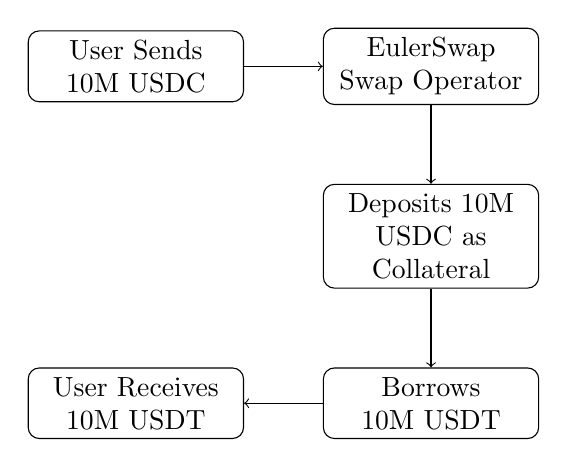
\begin{tikzpicture}[
        node distance=1cm, 
        every node/.style={draw, text width=2.5cm, align=center, rounded corners}
        ]
        % Nodes
        \node (user1) {User Sends 10M USDC};
        \node (EulerSwap) [right=of user1] {EulerSwap Swap Operator};
        \node (deposit) [below=of EulerSwap] {Deposits 10M USDC as Collateral};
        \node (borrow) [below=of deposit] {Borrows ~10M USDT};
        \node (user2) [left=of borrow] {User Receives 10M USDT};
        
        % Arrows
        \draw[->] (user1) -- (EulerSwap);
        \draw[->] (EulerSwap) -- (deposit);
        \draw[->] (deposit) -- (borrow);
        \draw[->] (borrow) -- (user2);
    \end{tikzpicture}
    \caption{\textbf{Swap flow in EulerSwap AMM}. EulerSwap’s just-in-time liquidity borrowing. The swap operator dynamically increases liquidity by borrowing the ``out token" against the ``in token."}
    \label{fig:EulerSwap_liquidity}
\end{figure}

\section{Virtual reserves and debt limits}

Since EulerSwap AMMs do not hold the assets used to service swaps at all times, they do swap calculations based on `virtual' reserves and debt limits, rather than on `real' reserves. 

Each EulerSwap LP can configure independent virtual reserve levels. These reserves define the maximum debt exposure an AMM will take on. For instance, if a user deposits \$1,000 in collateral and sets virtual reserves at \$5,000 per vault, the AMM effectively supports up to \$10,000 in combined swap depth, with a loan-to-value (LTV) ratio of 83.3\%. 

Note that the effective LTV must always remain below the borrowing LTV of the credit vault to prevent liquidation. Additionally, different AMM curves influence whether the maximum virtual reserves are achievable.

\section{Curve}

The space of possible reserves in an EulerSwap AMM is determined by how much debt a swap operator is allowed to hold. The EulerSwap curve passes through an equilibrium point $(x_0, y_0)$, at which the marginal price is defined by:

\begin{equation}
\frac{dy}{dx} \Big|_{(x_0, y_0)} = -\frac{p_x}{p_y}.
\end{equation}

Unlike most AMM curves, which are usually defined by a single convex function, EulerSwap uses a piecewise-defined curve, with different functions providing trading behaviour either side of the equilibrium point:

\begin{equation}
    \label{eq:fx-main}
    f(x) =
    \begin{dcases}
        f_1(x), 
        & 0 < x \leq x_0 \\
        f_2(x), 
        & x_0 < x
    \end{dcases}.
\end{equation}

In the domain $0 < x \leq x_0$, the curve is defined by

\begin{equation}
    \label{eq:fx1-main}
    f_1(x) 
    =
    y_{0}+\frac{p_{x}}{p_{y}}\left(x_{0}-x\right)\left(c_{x}+\left(1-c_{x}\right)\left(\frac{x_{0}}{x}\right)\right).
\end{equation}

In the domain $x_0 < x$, the curve is defined by

\begin{equation}
    \label{eq:fx2-main}
    f_2(x) 
    =
    \frac{
        \sqrt{
            \left( \frac{p_x}{p_y} (x - x_0) + y_0 (1 - 2c_y) \right)^2 
            + 4c_y (1 - c_y) y_0^2
        } 
        - \left( \frac{p_x}{p_y} (x - x_0) + y_0 (1 - 2c_y) \right)
    }{2c_y}.
\end{equation}

 The $c_x, c_y$ parameters here are liquidity concentration parameters that control how liquidity is distributed along the curve, with values closer to 1 concentrating liquidity around equilibrium and values closer to 0 distributing it across a wider price range. This flexibility enables EulerSwap to be used for entirely new use cases or to simulate the behaviour of atypical AMM protocols, such as the MakerDAO \href{https://mips.makerdao.com/mips/details/MIP29}{Peg Stability Module} (PSM). A full derivation is given in the Appendix \ref{sec:appendix}.  
 
 \begin{figure}[h]  % 'h' places it here, 't' for top, 'b' for bottom, 'p' for separate page
    \centering  % Centers the image
    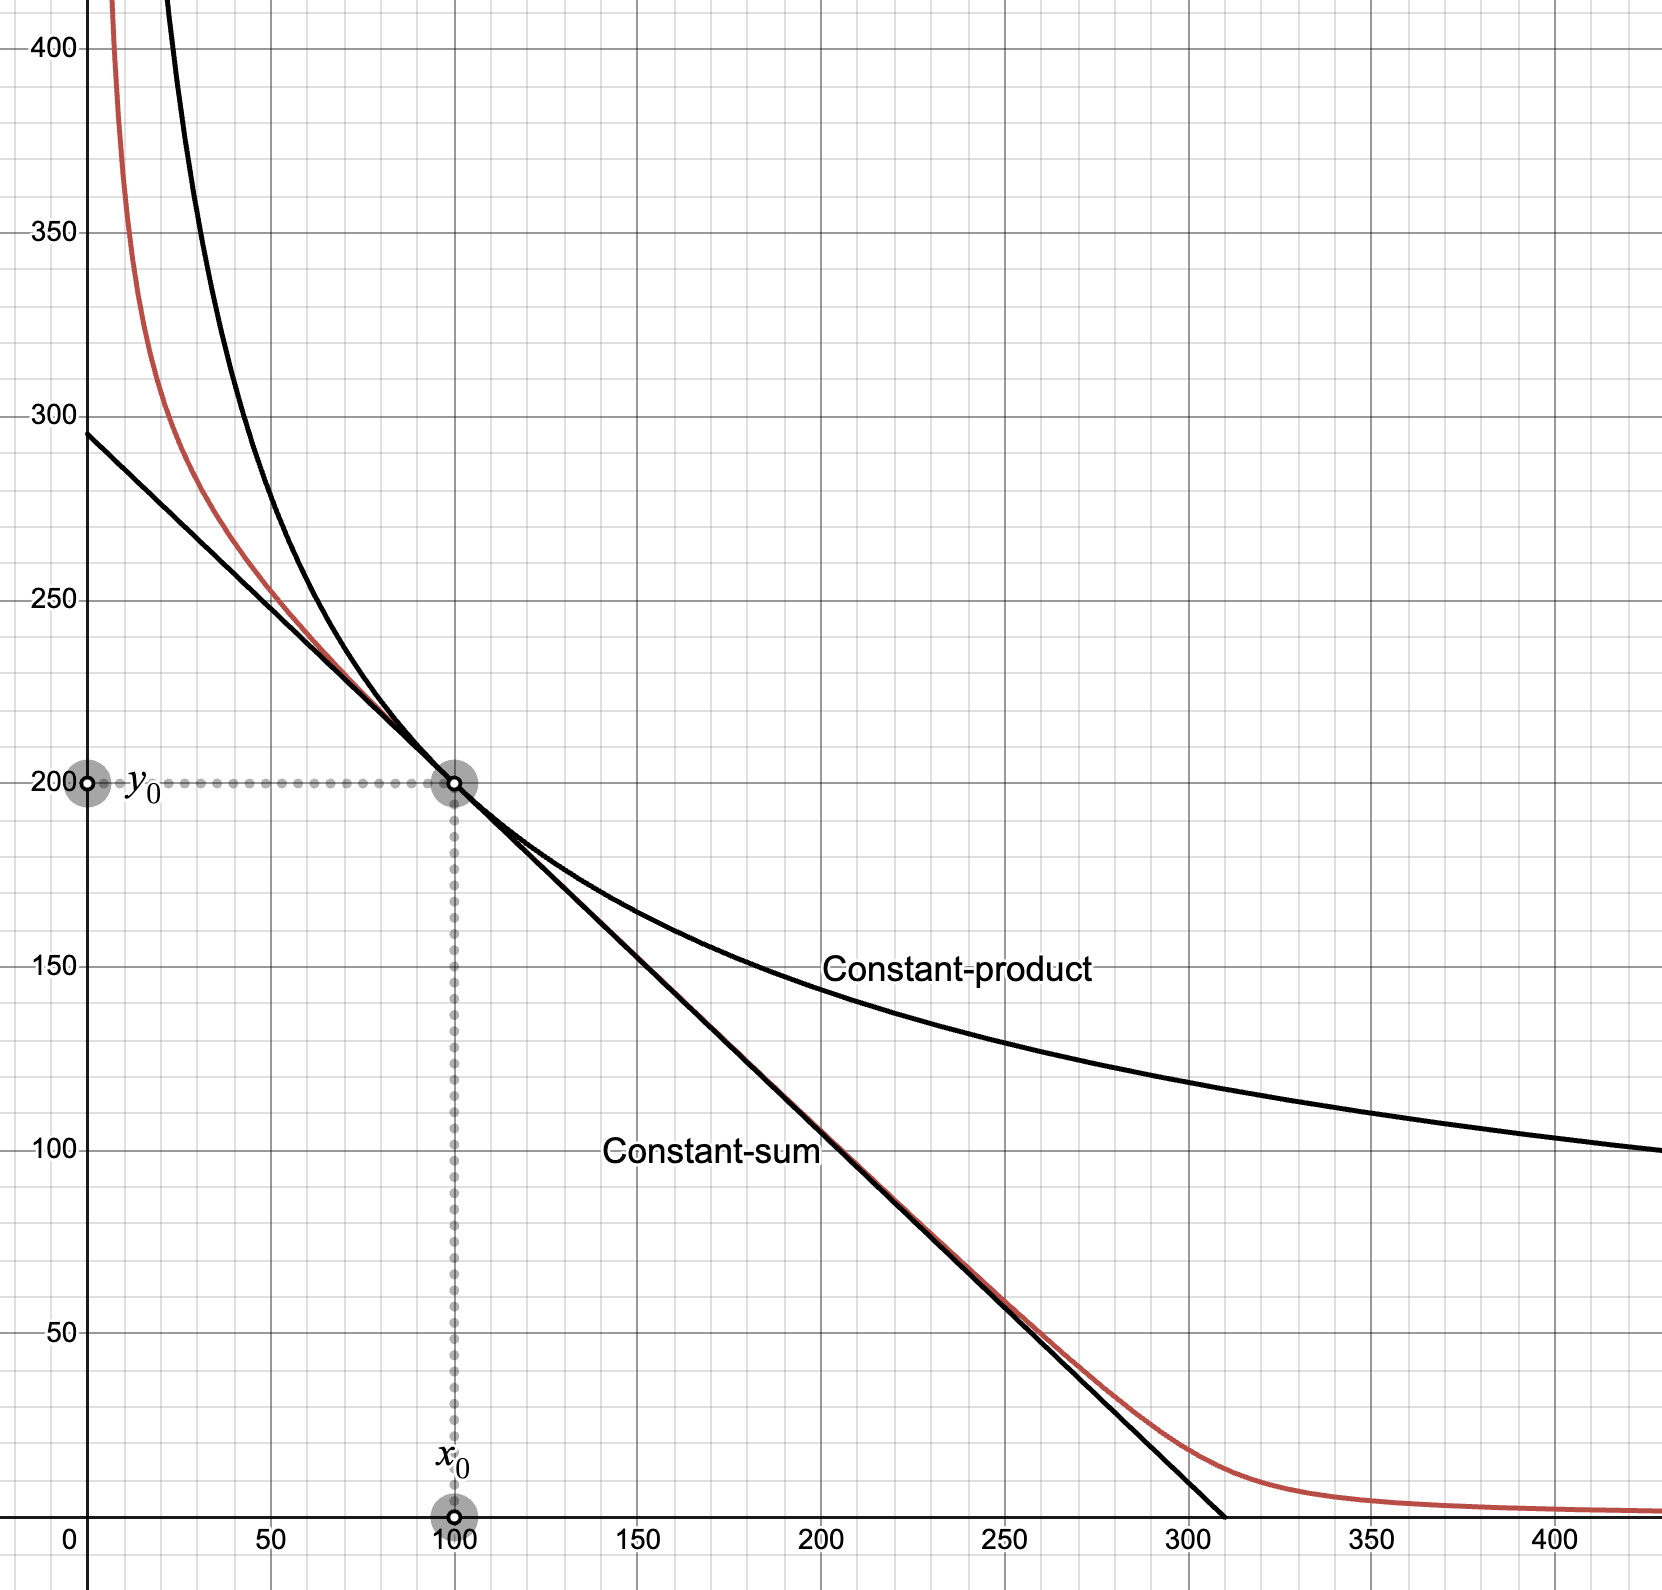
\includegraphics[width=0.5\textwidth]{curve.png} % Adjust width as needed
    \caption{\textbf{EulerSwap AMM curve.} The EulerSwap curve (red line) consists of two sides with separate reserve values $x_0, y_0$ and liquidity concentration parameters $c_x, c_y$, allowing liquidity to be distributed asymmetrically. This means liquidity can be more or less dense or concentrated on one side of the AMM relative to the other. The exchange rate at equilibrium is determined by the pricing parameters $p_x, p_y$ and is fully flexible. You can interact with the curve \href{https://www.desmos.com/calculator/gzwmvbs1dk}{here} on Desmos to compare its behaviour with traditional constant-sum and constant-product curves (black lines).}
    \label{fig:fig1}  % Useful for referencing the figure in text
\end{figure}

\section{Conclusion}

EulerSwap enhances AMMs by leveraging just-in-time liquidity to expand the depth of liquidity available to swappers. By integrating Euler’s credit vaults, it enables LPs to earn swap fees on top of their ordinary deposits while offering a customisable AMM curve that supports concentrated, distributed, and asymmetric liquidity structures. These features make EulerSwap adaptable to a wide range of trading strategies. However, this efficiency is not without some trade-offs. Swap operators incur interest costs on borrowed assets, which can erode profitability if not offset by swap fees, interest on collateral, or token incentives. Additionally, EulerSwap inherits Euler’s risk parameters, making it most effective for correlated asset pairs with high loan-to-value (LTV) ratios, while volatile assets pose higher liquidation risks if positions become imbalanced. Despite these trade-offs, EulerSwap represents a breakthrough in AMM design by repurposing idle liquidity in lending protocols, reducing capital inefficiencies, and optimising swap execution. By catering to professional market makers, DAOs, and algorithmic traders, it positions itself as a powerful tool for on-chain liquidity optimisation. Future research could explore optimal strategies for setting pricing and liquidity concentration parameters dynamically based on market conditions. EulerSwap's design opens new possibilities for AMM efficiency, setting a foundation for further DeFi innovation.

\section*{Acknowledgments}

During a security review of EulerSwap, Chris Michel noted similarities between some of its underlying concepts and BlackHoleSwap, a project prototype he had reviewed years earlier. While EulerSwap was designed independently and without influence from that project, the resemblance is significant enough to warrant its recognition here as prior art.

\newpage
\section{Appendix}
\label{sec:appendix}

\subsection{Curve derivation}
\label{sec:curve-derivation}

We begin with an Automated Market Maker (AMM) holding initial liquidity reserves of two assets, $X$ and $Y$, denoted as $x_0$ and $y_0$, respectively. In the absence of trading, the AMM remains at equilibrium at the point $(x_0, y_0)$. 

Our goal is to derive a curve for a constant-function trading market maker (CFMM) that supports swaps between the two assets with the following properties:

\begin{itemize}
    \item Passes through the equilibrium point $(x_0, y_0)$.
    \item Maintains an exchange rate, given by the slope of the AMM curve, of $-p_x / p_y$ at $(x_0, y_0)$.
    \item Allows liquidity concentration to be adjusted via parameters $c_x$ and $c_y$, which control the liquidity available for swaps to the left and right of the equilibrium point.
\end{itemize}

To develop such a function, we first introduce two fundamental AMM curve models.

\subsubsection{Constant-sum and constant-product AMM curves}

The canonical constant-sum (CSMM) and constant-product (CPMM) market making curves are given by:

\begin{align}
    x + y &= x_0 + y_0, \\
    xy &= x_0 y_0.
\end{align}

The CSMM is simply a line, whilst the CPMM is a hyperbola. These curves can be thought of as two extremes when it comes to the distribution of liquidity. The CSMM concentrates liquidity at a single exchange rate, whilst the CPMM distributes liquidity across a wide range of different exchange rates. By default, these curves intersect at the equilbirium point $(x_0, y_0)$, where their slopes are:

\begin{align}
    \frac{dy}{dx} &= -1, \\
    \frac{dy}{dx} &= -\frac{y}{x}.
\end{align}

Since real-world markets often operate at variable exchange rates at equilibrium, we introduce custom pricing parameters $p_x$ and $p_y$ to allow flexibility in defining the slope at the equilibrium point:

\begin{align}
    \label{eq:weighted-line}
    p_x x + p_y y &= p_x x_0 + p_y y_0, \\
    \label{eq:exponential-form}
    x^{p_y y_0} y^{p_x x_0} &= x_0^{p_y y_0} y_0^{p_x x_0}.
\end{align}

The CSMM is now a line with a slope parameterised by the ratio of the pricing parameters, whilst the CPMM is now a \textit{weighted} hyperbola. Taking the derivatives of these equations with respect to $x$, we obtain:

\begin{align}
    \frac{dy}{dx} &= -\frac{p_x}{p_y}, \\
    \frac{dy}{dx} &= -\frac{p_x}{p_y} \frac{x_0 y}{y_0 x}.
\end{align}

These results confirm that at equilibrium $(x_0, y_0)$, the slope of both functions is:

\[
\frac{dy}{dx} \Big|_{(x_0, y_0)} = -\frac{p_x}{p_y}.
\]

Whilst these curves sufficiently generalise the constant-sum and constant-product curves to an arbitrary price at equilibrium, in practice, the modified CPMM equation \eqref{eq:exponential-form} has limited practical application as a CFMM because it involves an exponential form that is computationally intensive and impractical for on-chain calculations. We therefore seek a simpler equation that preserves the spirit of the trading behaviour of the generalised CPMM; that is, some kind of herpbola that passes through the equilibrium point $(x_0, y_0)$ and maintains an exchange rate of $-p_x / p_y$ at that point. To resolve this, we introduce the concept of artificial reserves.

\subsubsection{Introducing artificial reserves to create a new, simpler curve}

Note that in the interval $0 < x < x_0$ swaps should only increase liquidity beyond $y_0$ and deplete $x_0$ liquidity. That is, our trading function in this interval need not depend on the initial amount of $y_0$ liquidity. This suggests that we can split the domain of the AMM curves into two, and replace the real reserve $y_0$ in the interval $0 < x < x_0$ with an carefully chosen artificial reserve $y_v$ designed to eliminate the exponential form in the weighted hyperbola. 

Re-arranging equations \eqref{eq:weighted-line} and \eqref{eq:exponential-form} into explicit functions of $y$, we obtain
\begin{align}
    \label{eq:weighted-line-explicit}
    y &= y_0 + \frac{p_x}{ p_y} (x_0 - x), \\
    \label{eq:exponential-form-explicit}
    y &= y_0 \left( \frac{x_0}{x} \right)^{\frac{p_y y_0}{p_x x_0}}.
\end{align}

In this view, it is easy to see that a substitution of $y_0 \rightarrow y_v$, given by

\[
y_v = x_0 \frac{p_x}{p_y}.
\]

will eliminate the exponential form in equation \eqref{eq:exponential-form-explicit}. We then have equations

\begin{align}
    y &= \frac{p_x}{p_y} (2x_0 - x), \\
    y &= \frac{p_x}{p_y} \frac{x_0^2}{x}.
\end{align}

Note that simply shifting the curve up or down does not impact the slope or shapes of the curves and therefore has no impact on trading behaviour. Since these curves no longer pass through \( (x_0, y_0) \), we therefore correct them by adding back the difference \( y_0 - p_x / p_y x_0 \). This leads to:

\begin{align}
    y &= y_0 + \frac{p_x}{p_y} (x_0 - x), \\
    y &= y_0 + \frac{p_x}{p_y} (x_0 - x) \left( \frac{x_0}{x} \right).
\end{align}

Taking the derivatives of these equations with respect to $x$, we obtain:

\begin{align}
    \frac{dy}{dx} &= -\frac{p_x}{p_y}, \\
    \frac{dy}{dx} &= -\frac{p_x}{p_y} \left( \frac{x_0}{x} + \frac{x_0(x_0 - x)}{x^2} \right).
\end{align}

These results confirm that at equilibrium $(x_0, y_0)$, the slope of both functions is:

\[
\frac{dy}{dx} \Big|_{(x_0, y_0)} = -\frac{p_x}{p_y}.
\]

\subsubsection{Unifying into a single curve in the region $0 < x < x_0$}

To create a single unified curve, we introduce a liquidity concentration parameter \( c_x \in [0, 1] \), which determines the curve’s behaviour:

\begin{itemize}
    \item When \( c_x = 1 \), the AMM functions as a constant-sum AMM.
    \item When \( c_x = 0 \), the AMM behaves as a constant-product-like AMM.
    \item Intermediate values of \( c_x \) create a hybrid trading function with liquidity that is more or less concentrated around the equilibrium point.
\end{itemize}

This gives the final equation:

\begin{equation}
    \label{eq:EulerSwap-1}
    y = y_0 + \frac{p_x}{p_y} (x_0 - x) \left( c_x + (1 - c_x) \left(\frac{x_0}{x}\right) \right).
\end{equation}

This is equivalent to the function \( f_1(x) \) given by equation \eqref{eq:fx1-main} in the main text.

\subsubsection{Extending the curve to the $x > x_0$ region}

It is important to remember that equation \eqref{eq:EulerSwap-1} only works as a trading function in the interval $0 < x < x_0$. For \( x > x_0 \), we construct a reflected curve that also passes through \( (x_0, y_0) \) and maintains the required derivative:

\begin{equation}
    \label{eq:EulerSwap-3-inverse}
    x = x_0 + \frac{p_y}{p_x} (y_0 - y) \left( c_y + (1 - c_y) \left(\frac{y_0}{y}\right) \right).
\end{equation}

Since this equation defines \( x \) in terms of \( y \), we invert it by solving for \( y \), leading to the quadratic equation:

\begin{equation}
    y = c_y y^2 + \left( \frac{p_x}{p_y} (x - x_0) - y_0(2c_y - 1) \right)y - (1 - c_y) y_0^2.
\end{equation}

Taking only the positive real root, we obtain:

\begin{equation}
    \label{eq:EulerSwap-2}
    y = \frac{
        \sqrt{
            \left( \frac{p_x}{p_y} (x - x_0) + y_0 (1 - 2c_y) \right)^2 
            + 4c_y (1 - c_y) y_0^2
        } 
        - \left( \frac{p_x}{p_y} (x - x_0) + y_0 (1 - 2c_y) \right)
    }{2c_y}.
\end{equation}

This corresponds to the function \( f_2(x) \) given by equation \eqref{eq:fx2-main} in the main text.

\subsection{Invariant derivation}
\label{sec:invariant-derivation}

In traditional AMM protocols, the curve is typically defined as an implicit function of $y$. For example, the classic Uniswap AMM follows a constant-product equation:

\begin{equation}
    xy = x_0 y_0
\end{equation}

where $x_0$ and $y_0$ are the initial liquidity reserves. This equation defines an invariant condition, ensuring that any valid swap must satisfy:

\begin{equation}
    xy \geq x_0 y_0.
\end{equation}

This condition guarantees that after any trade, the product of the new reserves remains at least as large as the initial product, ensuring that swaps cannot drain liquidity from the pool.

Rearranging this condition, we can express the invariant as a lower bound for $y$:

\begin{equation}
    y \geq \frac{x_0 y_0}{x}.
\end{equation}

This means that for any valid trade, the resulting reserve state must lie on or above the AMM curve.  

\subsubsection{Extending the invariant to EulerSwap}

For EulerSwap, we apply a similar principle. Given any reserve state $(x, y)$, we check whether it satisfies an equivalent invariant condition.

From equation \eqref{eq:EulerSwap-1}, for values where \( 0 < x < x_0 \), the AMM curve constraint requires:

\begin{equation}
    \label{eq:invariant-x1}
    y \geq y_{0}+\frac{p_{x}}{p_{y}}\left(x_{0}-x\right)\left(c_{x}+\left(1-c_{x}\right)\left(\frac{x_{0}}{x}\right)\right).
\end{equation}

For values where \( x > x_0 \), we could derive a similar condition for $y$ from equation \eqref{eq:EulerSwap-2}. However, a simpler and computationally cheaper approach is to use the inverse equation \eqref{eq:EulerSwap-3-inverse}, which defines the lower bound for $x$ instead:

\begin{equation}
    \label{eq:invariant-x2}
    x \geq x_{0}+\frac{p_{y}}{p_{x}}\left(y_{0}-y\right)\left(c_{y}+\left(1-c_{y}\right)\left(\frac{y_{0}}{y}\right)\right).
\end{equation}

These conditions together define the valid liquidity states in EulerSwap, ensuring that the AMM remains balanced while allowing for greater flexibility in liquidity provisioning.

\section{Disclaimer}

This paper is for general information purposes only. It does not constitute investment
advice or a recommendation or solicitation to buy or sell any investment and should not
be used in the evaluation of the merits of making any investment decision. It should not
be relied upon for accounting, legal or tax advice or investment recommendations. This
paper reflects current opinions of the authors and is not made on behalf of Euler Labs or its
affiliates and does not necessarily reflect the opinions of Euler Labs, its affiliates or individuals
associated with Euler Labs. The opinions reflected herein are subject to change without being
updated.

\end{document}



Section 5.1.2 starts off with the principle that the trading function should not depend on y0, and applies it to formula (8), on the assumption (correct me if I'm wrong) that whatever y_v we choose will not change the trading behaviour. However this is not true for formula (8), because y0 is not just a vertical offset, but is embedded in the exponents.
What stays true is just the fact that, whatever y_v we choose, the curve will pass through the point (x0, y_v) with slope -px/py, so we might as well choose an "easy" one that simplifies the calculations: the driving reason for imposing px x0 = py yv seems rather to be that this renders the exponents in formula (8) equal, thus effectively reverting it to an unweighted hyperbola. Then, once we add back the vertical offset, the trading behaviour of formula (14) indeed no longer depends on y0, but just because we have now "made" y0 just a vertical offset, shifting formula (12). 
In other words, we have formula (8) which defines a parametric curve y = f(x; x*,y*,p*) that always passes through the point (x*,y*) with slope -p*. We want a function that passes through (x0,y0) with slope -p0. We could use y = f(x; x0,y0,p0) but this is computationally intensive. Instead, we choose y = f(x; x0,x0p0,p0) + (y0 - x0p0) because this still satisfies the requirements, but the particular choice of y* makes f() less computationally intensive.
In fact, there is a mistake earlier on in the appendix: the slope of the plain hyperbola x y = x0 y0 at the point (x0, y0) is not -1 but -y0/x0. The choice of y_v = x0 px/py makes that slope equal to -px/py. So overall it would seem like choosing a plain hyperbola from the start, with appropriate parameters and offset, would do the trick. Have I interpreted correctly the intentions of your derivation process?